
\section{在室者情報を用いた応用システムについて}\label{3.4}
部屋利用者の在室者情報を用いれば,部屋の管理者や部屋利用者にとって便利な応用システムが考えられる.
1つ目の応用システムとして,勤怠管理システムが考えられる.
勤怠管理システムの代表例としてタイムカードでの打刻や,ICカードやQRコード,スマートフォンによる記録が挙げられる.
これらのシステムでは利用者が能動的に記録する必要がある.
本研究でのビーコンを用いた手法では能動的な記録を必要とせず,自動で記録されるため,利用者の負担や記録のし忘れが減ると考えられる.
2つ目の応用システムとして,コミュニケーション促進システムが考えられる.
研究室では部屋利用者同士の活発なコミュニケーションが求められる.
しかし研究室に所属する部屋利用者は必ずしも共通の話題を持つ人が集まるわけではない.
そこで部屋利用者が共有できる情報である在室者情報を用いてコミュニケーションを促進するようなシステムを構築する.
コミュニケーション促進システムについては4章で実装した「きょうの滞在」で詳しく述べる.
3つ目の応用システムとして,来訪促進システムが考えられる.
在室者情報を用いたゲーミフィケーションに基づくシステムが考えられる.
具体例として在室履歴を用いたペット育成ゲームが考えられる.
在室履歴を用いたペット育成ゲームの概要を図\ref{petgaiyou}に示す.
部屋利用者の在室履歴からペットに餌を与えられるようなシステムである.
部屋利用者はペットに餌を与えるためには部屋に在室する必要がある.
そのためペットに愛着があるなら部屋利用者は来訪する必要がある.
また在室履歴を用いたペット育成ゲームのアプリのイメージ図を図\ref{petimage}に示す.
誰でも見やすいようなレイアウトやスマホでの利用を想定したボタン配置を意識した.
\begin{figure}[H]
  \begin{center}
    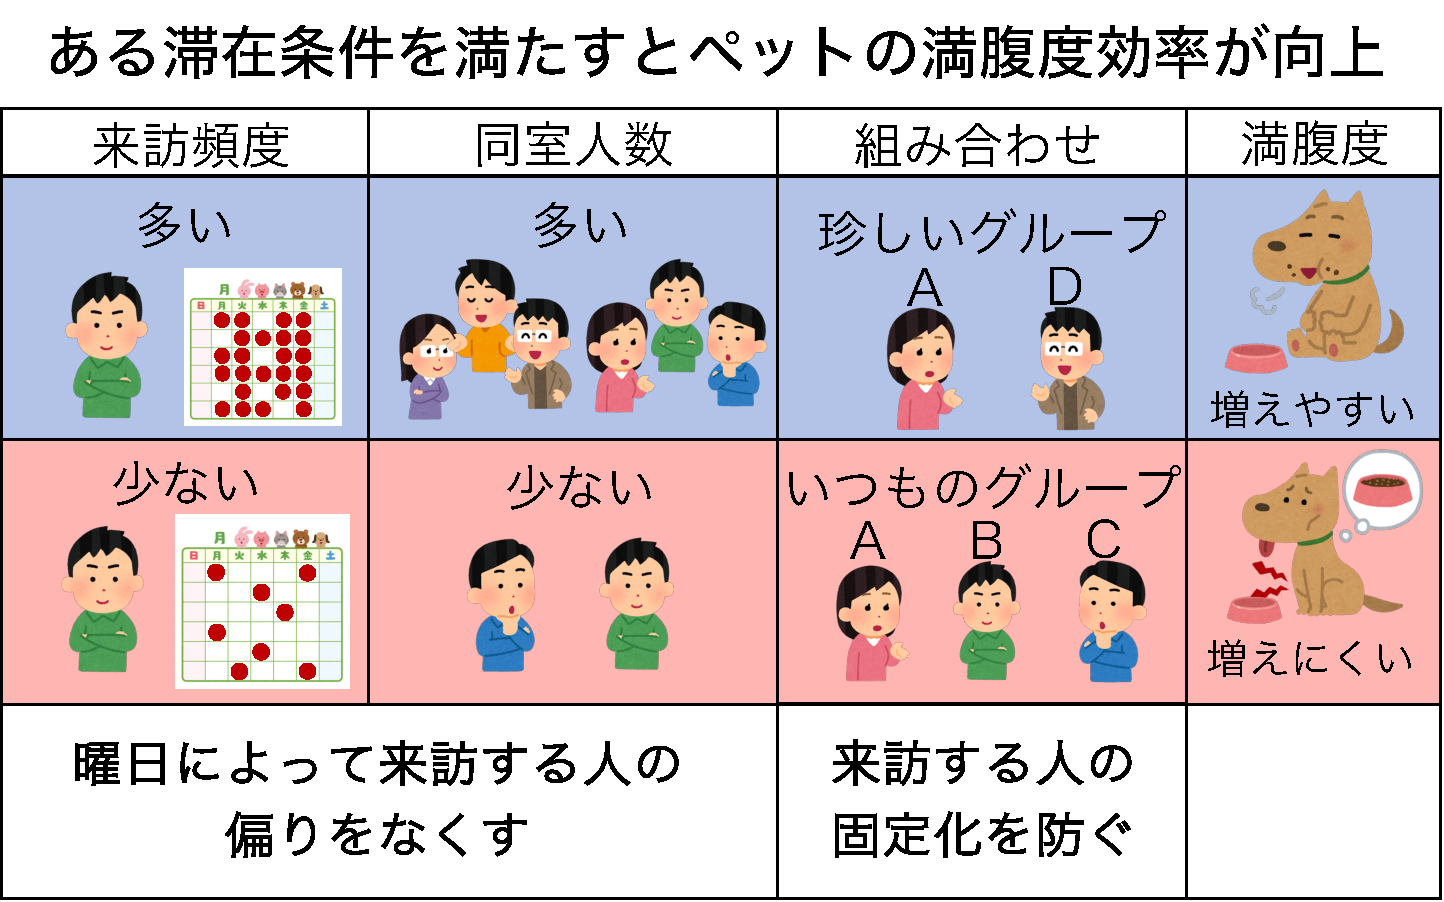
\includegraphics[width=160mm]{image/petgaiyou.pdf}
    \caption{来訪促進システムの概要図}
    \label{petgaiyou}
  \end{center}
\end{figure}

\begin{figure}[H]
  \begin{center}
    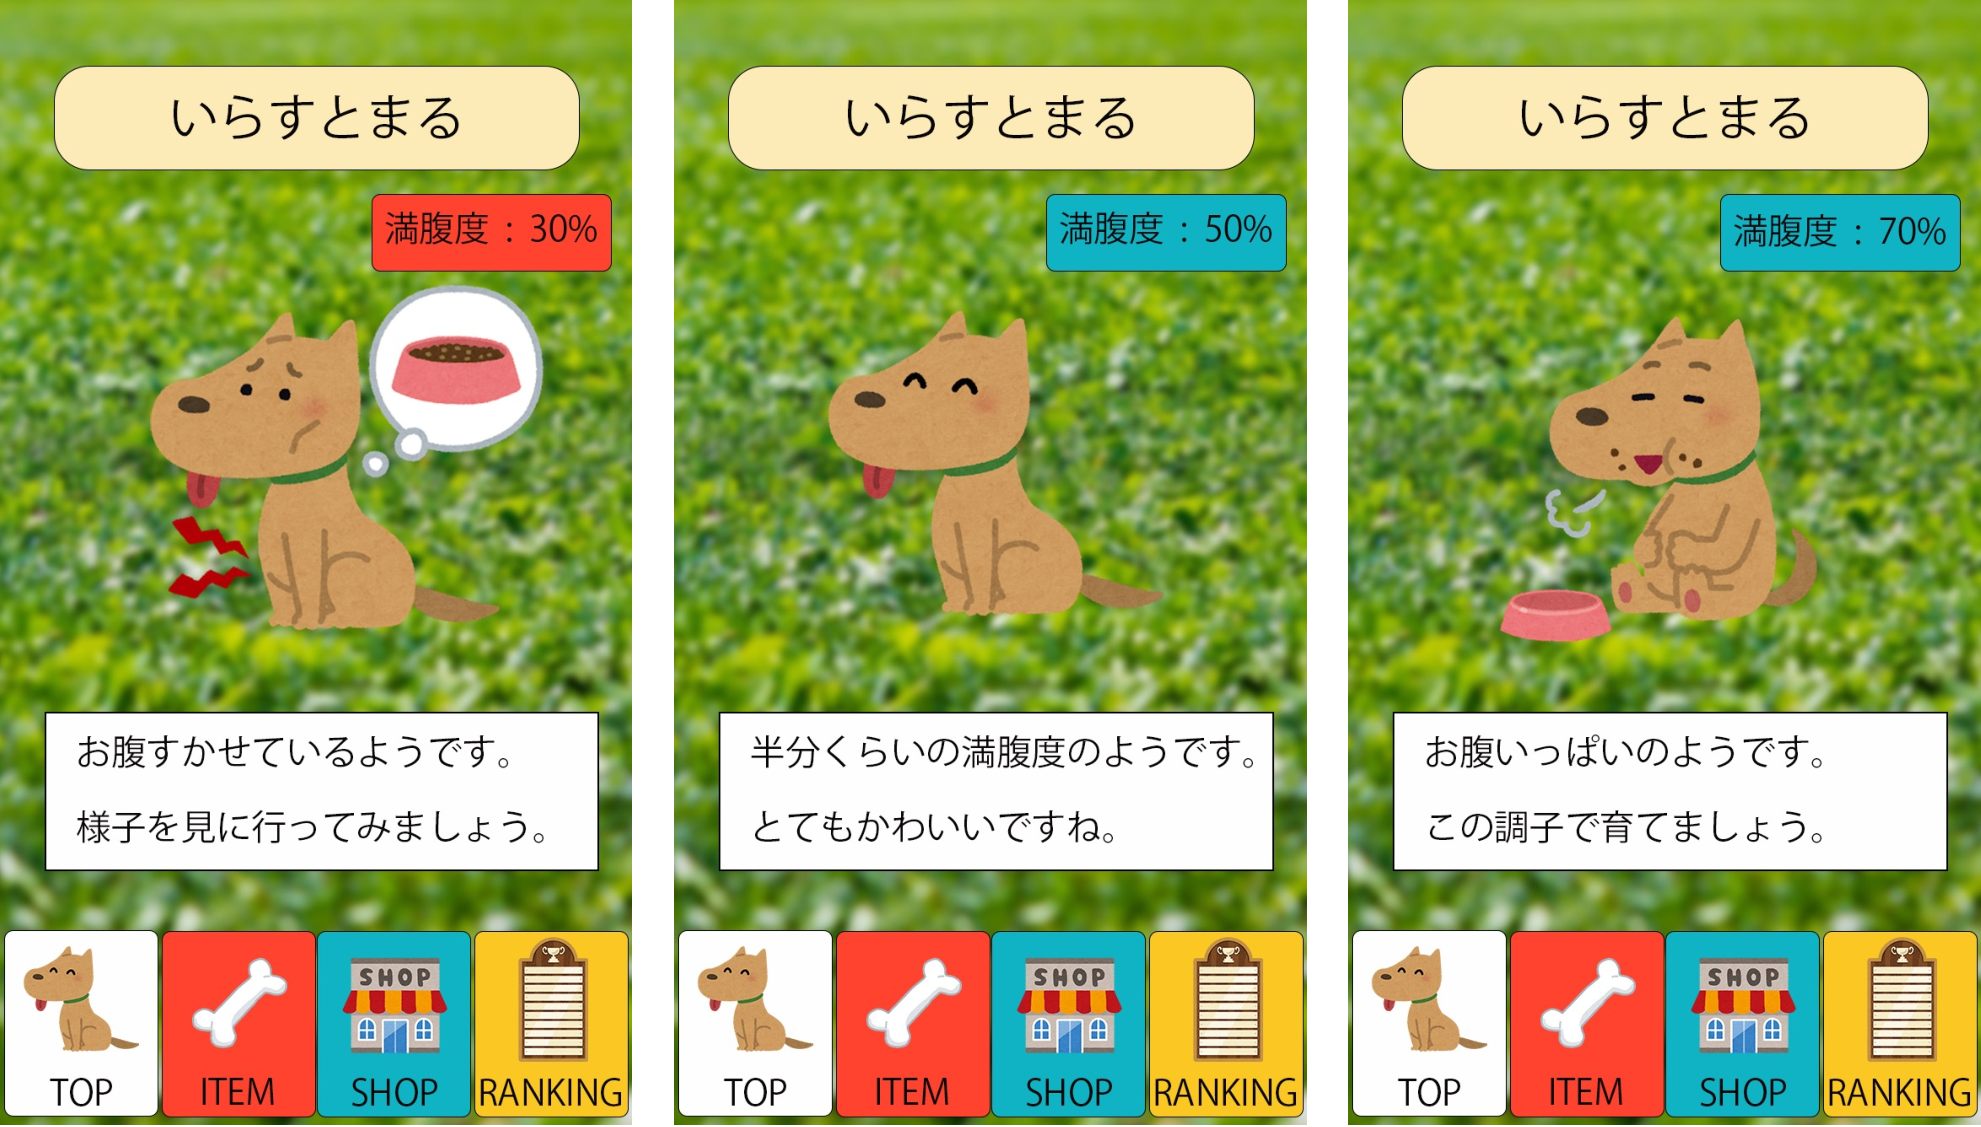
\includegraphics[width=160mm]{image/petimage.pdf}
    \caption{ペット育成ゲームのアプリのイメージ}
    \label{petimage}
  \end{center}
\end{figure}

\thispagestyle{myheadings}